\documentclass{article}
\usepackage[utf8]{inputenc}
\usepackage{color}
\usepackage{listings}
\usepackage{graphicx}
\lstset{
language=C++,
basicstyle=\footnotesize,
numbers=left,
numberstyle=\footnotesize,
stepnumber=1,
numbersep=5pt,
backgroundcolor=\color{white},
showspaces=false,
showstringspaces=false,
showtabs=false,
frame=single,
tabsize=2,
captionpos=b,
breaklines=true,
breakatwhitespace=false,
escapeinside={\%*}{*)}
}

\title{\textbf{ANALISIS Y DISEÑO DE ALGORITMOS}}
\author{\textbf{Jorge Alfredo Mayna Flores} \\
Universidad de Ingeniería y Tecnología}

\date{November, 2018}

\begin{document}

\maketitle
\section{Ejercicio 1}
En el merge sort clásico, se divide recursivamente un array en 2 partes iguales y se van ordenando hasta que todo el array este ordenado. Pero si dividir el problema en 2 da buenos resultados ¿porque no se podría partir en mas partes?.
\\
\\

El tiempo de ejecución al partirlo en 2 mitades es $O(n.log_{2}n)$ esto debido a que en cada paso la cadena se va partiendo en 2. Para una mayor cantidad de divisiones podríamos tener:
\begin{equation}
    T(n)=kT(n/k)+O(n)
\end{equation}
De este modo para el caso de 3 divisiones tendríamos: $T(n)=3T(n/3)+O(n)$ lo que equivaldría a  $O(n.log_{3}n)$. Sin embargo, ¿Es esto verdaderamente mejor?.\\
Dividirlo en 3 resulta en una implementación mas compleja y si bien reduces la cantidad de pasos recursivos aumentas el numero de comparaciones lo que podría llevar a hacerlo incluso mas lento.
\section{Ejercicio 2}
\begin{itemize}
    \item 3n + 1
\end{itemize}
\begin{lstlisting}
#include <iostream>
using namespace std;

int main ()
{
	int n1,n2;
	int mayor,menor;
	while(cin >> n1 >> n2){

		if(n1>n2){
            mayor=n1;
            menor=n2;
		}else{
            mayor=n2;
            menor=n1;
		}
		int largo;
		int n_largo=0;

		for(int i=menor; i<=mayor; i++)
		{
			int ev=i;
			largo=1;

			while(ev !=1 )
			{
				if(ev%2 != 0){
				     ev = ev*3 +1;
				     largo++;
                }else {
                    ev=ev/2;
                    largo++;
				}
			}
			if(largo>n_largo){
                n_largo=largo;
			}
		}

		cout << n1<<" " <<n2<< " "<<n_largo<< endl;
	}
    return 0;
}
\end{lstlisting}

\section{Ejercicio 3}
*Codigo completo anexado al archivo
\begin{itemize}
    \item Implementación de Insertion Sort:
\end{itemize}
\begin{lstlisting}
void insertion_sort(int* _array,int n){
    int key,j;
    for(int i=1;i<n;i++){
        key=_array[i];
        j=i-1;
        while(j>=0 && _array[j]>key){
            _array[j+1]=_array[j];
            j=j-1;
        }
        _array[j+1]=key;
    }
}
\end{lstlisting}

\begin{itemize}
    \item Implementación de Merge Sort:
\end{itemize}

\begin{lstlisting}
void merge_sort(int* _array,int i,int d){
    if(d>i){
        int me = (d+i)/2;
        merge_sort(_array,i,me);
        merge_sort(_array,me+1,d);
        Merge(_array,i,me,d);

    }
}
\end{lstlisting}

\begin{lstlisting}
void Merge(int* _array,int i,int me,int d){
    int n1= me-i +1;
    int n2= d-me;
    int l[n1+1],r[n2+1];
    for(int z=0;z<n1;z++){
        l[z]=_array[i+z];
    }
    for(int z=0;z<n2;z++){
        r[z]=_array[me+1+z];
    }
    l[n1]=INF;
    r[n2]=INF;
    int z=0,x=0,k=i;
    while(z!=n1 || x!=n2){
        if(l[z]<=r[x]){
            _array[k]=l[z];
            z++;
        }else{
            _array[k]=r[x];
            x++;
        }
        k++;
    }
}
\end{lstlisting}

Para las comparaciones entre los 2 algoritmos evalué el peor caso posible, para lo cual generé automáticamente arrays en orden descendente los cuales fueron reordenados con cada uno de los algoritmos 10 000 veces para luego obtener un promedio del tiempo medido.\\
Se repitió este proceso para arrays desde tamaño 1 hasta tamaño 500 y guarde los resultados en un .txt(*Anexado a este archivo).\\
Con los datos obtenidos se uso la librería gnuplot y se grafico el documento de texto con el siguiente comando:
\begin{itemize}
    \item plot  'record.txt'  using 0:2 with lines,'' using 0:3 with lines
\end{itemize}
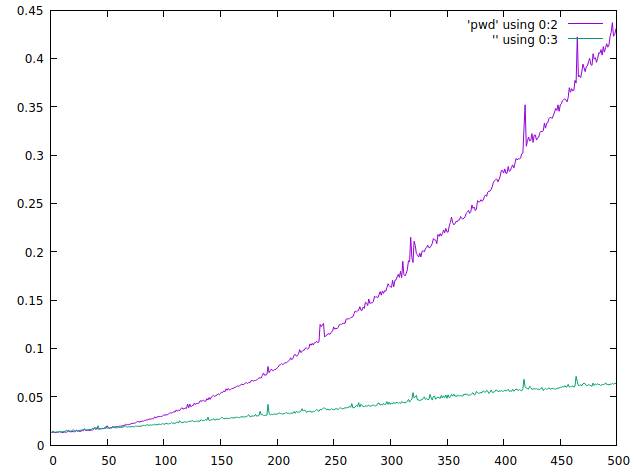
\includegraphics[width=\textwidth]{500datos.PNG}\\
Para poder observar mejor el punto donde el merge sort se vuelve mejor que el insert sort se redujo el tamaño de nuestro txt a solo 100 datos:\\
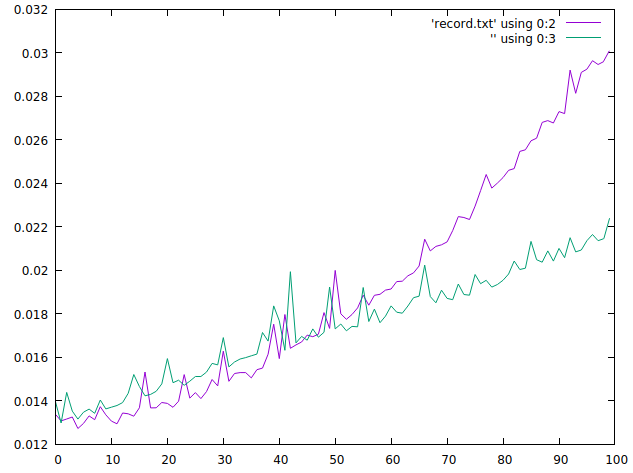
\includegraphics[width=\textwidth]{100datos.PNG}\\

En el gráfico se pudo apreciar que si bien el insertion sort comienza teniendo mejor tiempo de ejecución, alrededor del tamaño 40-45 el merge sort lo empieza a sobrepasar y posteriormente le saca mucha ventaja.
\section{Pregunta 4}
El algoritmos de karatsuba sirve para reducir el costo computacional al realizar multiplicaciones muy grandes. Logra reducir la complejidad del metodo clasico de multiplicar($O(n^2)$) a como maximo $3n^{log_23}$ multiplicaciones de un dígito.\\
El algoritmo convierte la multiplicación de 2 números grandes en 3 multiplicaciones de números mas pequeños(además de unas sumas y restas) las cuales se pueden resolver recursivamente con el mismo método.\\
Tiene la siguiente forma:\\
$2883 = 28 x 10^2 + 83$\\
$1557 = 15 x 10^2 + 57$\\
$S0=28 x 15$\\
$S1=83 x 57$\\
$S2=(28+83)(15+57) - S0 - S1 $\\
$Respuesta=S0 x 10^{2x2} + S2 x 10^2 + S1$\\

\section{Pregunta 5}

Si analizamos los tiempos de las funciones dadas y las ordenamos de menor a mayor tendríamos:
\begin{itemize}
    \item $n^l^o^g^(^n^)$
    \item $n^2$
    \item $n^2logn$
    \item $2^n$
    \item $2^{2^n}$
\end{itemize}\\
Si gráficos las funciones se puede apreciar mas claramente:\\
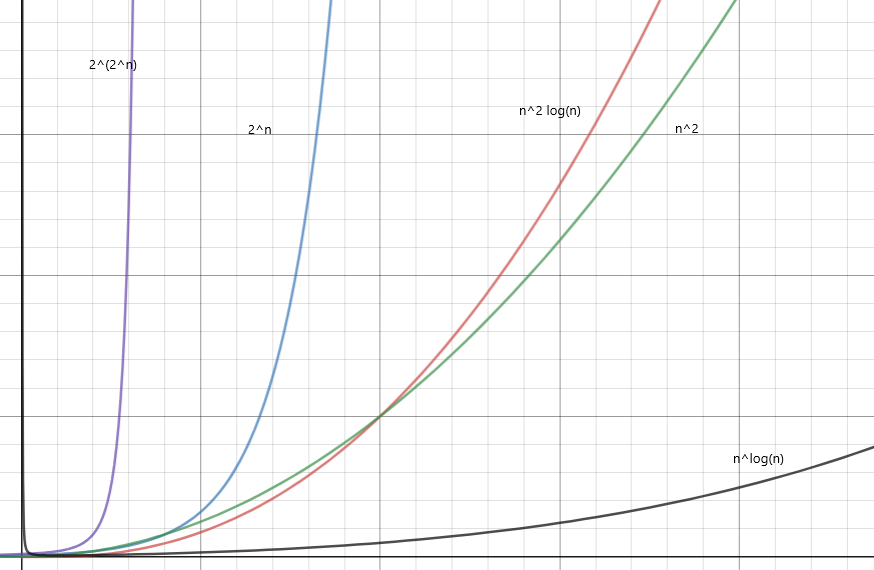
\includegraphics[width=\textwidth]{grafica.png}\\





\end{document}

%-------------------------------------------------------------------------------
% SNIPPETS
%-------------------------------------------------------------------------------

%\begin{figure}[!ht]
%	\centering
%	\includegraphics[width=0.8\textwidth]{file_name}
%	\caption{}
%	\centering
%	\label{label:file_name}
%\end{figure}

%\begin{figure}[!ht]
%	\centering
%	\includegraphics[width=0.8\textwidth]{graph}
%	\caption{Blood pressure ranges and associated level of hypertension (American Heart Association, 2013).}
%	\centering
%	\label{label:graph}
%\end{figure}

%\begin{wrapfigure}{r}{0.30\textwidth}
%	\vspace{-40pt}
%	\begin{center}
%		\includegraphics[width=0.29\textwidth]{file_name}
%	\end{center}
%	\vspace{-20pt}
%	\caption{}
%	\label{label:file_name}
%\end{wrapfigure}

%\begin{wrapfigure}{r}{0.45\textwidth}
%	\begin{center}
%		\includegraphics[width=0.29\textwidth]{manometer}
%	\end{center}
%	\caption{Aneroid sphygmomanometer with stethoscope (Medicalexpo, 2012).}
%	\label{label:manometer}
%\end{wrapfigure}

%\begin{table}[!ht]\footnotesize
%	\centering
%	\begin{tabular}{cccccc}
%	\toprule
%	\multicolumn{2}{c} {Pearson's correlation test} & \multicolumn{4}{c} {Independent t-test} \\
%	\midrule	
%	\multicolumn{2}{c} {Gender} & \multicolumn{2}{c} {Activity level} & \multicolumn{2}{c} {Gender} \\
%	\midrule
%	Males & Females & 1st level & 6th level & Males & Females \\
%	\midrule
%	\multicolumn{2}{c} {BMI vs. SP} & \multicolumn{2}{c} {Systolic pressure} & \multicolumn{2}{c} {Systolic Pressure} \\
%	\multicolumn{2}{c} {BMI vs. DP} & \multicolumn{2}{c} {Diastolic pressure} & \multicolumn{2}{c} {Diastolic pressure} \\
%	\multicolumn{2}{c} {BMI vs. MAP} & \multicolumn{2}{c} {MAP} & \multicolumn{2}{c} {MAP} \\
%	\multicolumn{2}{c} {W:H ratio vs. SP} & \multicolumn{2}{c} {BMI} & \multicolumn{2}{c} {BMI} \\
%	\multicolumn{2}{c} {W:H ratio vs. DP} & \multicolumn{2}{c} {W:H ratio} & \multicolumn{2}{c} {W:H ratio} \\
%	\multicolumn{2}{c} {W:H ratio vs. MAP} & \multicolumn{2}{c} {\% Body fat} & \multicolumn{2}{c} {\% Body fat} \\
%	\multicolumn{2}{c} {} & \multicolumn{2}{c} {Height} & \multicolumn{2}{c} {Height} \\
%	\multicolumn{2}{c} {} & \multicolumn{2}{c} {Weight} & \multicolumn{2}{c} {Weight} \\
%	\multicolumn{2}{c} {} & \multicolumn{2}{c} {Heart rate} & \multicolumn{2}{c} {Heart rate} \\
%	\bottomrule
%	\end{tabular}
%	\caption{Parameters that were analysed and related statistical test performed for current study. BMI - body mass index; SP - systolic pressure; DP - diastolic pressure; MAP - mean arterial pressure; W:H ratio - waist to hip ratio.}
%	\label{label:tests}
%\end{table}